% Chapter X

\chapter{Closure laws for the Heat Flux Partitioning model} % Chapter title

\label{ch:HFP_closures} % For referencing the chapter elsewhere, use \autoref{ch:name} 

%----------------------------------------------------------------------------------------

\minitoc


\section{Single-Phase Heat Transfer Coefficient}
\label{sec:single_phase_HTC}

The choice of a proper correlation to compute the single-phase heat transfer coefficient is a first but inevitable step to build a HFP model. Indeed, if the single-phase convection term is badly computed, the resulting boiling model will fail to predict the wall temperature.

For instance, if the liquid convective HTC is overestimated, it would result in a delayed increase of the boiling and quenching heat fluxes which would in turn lead to an overprediction of the wall temperature. 

To assess existing correlations for the single-phase HTC, we will use wall temperature measurements extracted from experimental boiling curves for water where $T_{w}\leq T_{sat}$. They correspond to the single-phase part of the experimental data later used to assess the HFP model.

The chosen data are presented on Table \ref{tab:exp_data_convection}.

\begin{table}[h!]

%\begin{changemargin}{-1cm}{0cm}

\noindent\makebox[\textwidth]{

\scriptsize
\centering
\begin{tabular}{p{20mm}|c c c c c c c c} 
Author & $D_{h}$ [mm] & $P$ [bar] & $G_{L}$ [$\debm$] & $\Delta T_{L}$ [K] & $\phi_{w}$ [MW/m\up{2}] & $T_{sat}-T_{w}$ [K] &$N_{mes}$ [-] \\
\hline
\\

Kossolapov \cite{kossolapov_experimental_2021} \newline (2021) & 12 & 10.5 & 500 - 2000 & 10 & 0.1 - 0.6  & 0.22 - 9.5 & 12 \\

Richenderfer \cite{richenderfer_phd} \newline (2018) & 15 & 1 - 5 & 1000 - 2000 & 10-20 & 0.1 - 0.63 & 1 - 18.7 & 13 \\

Jens-Lottes \cite{jens_lottes_data} \newline (1951) & 5.74 & 137.9 & 2617.5 & 53.3 - 92.2 & 0.91 - 2.37 & 0.33 - 44.1 & 15 \\

Kennel \cite{kennel_phd} \newline (1948) & 4.3 - 13.2 & 2 - 6.2 & 284 - 10~577 & 11.1 - 83.3 & 0.035 - 1.89 & 0.35 - 69 & 52 \\
\hline
\end{tabular}
}
\caption{Experimental data range of wall temperature measurements from the single-phase part of boiling curves.}
\label{tab:exp_data_convection}
\end{table}


On Figure \ref{fig:dittus_gniel_htc}, we compare the results of wall temperature prediction in the single-phase region obtained with the correlation of Dittus-Boelter (Eq. \ref{eq:dittus}) and Gnielinski (Eq. \ref{eq:gnielinski}).

\begin{figure}[h!]
\centering
\subfloat[Dittus-Boelter correlation]{
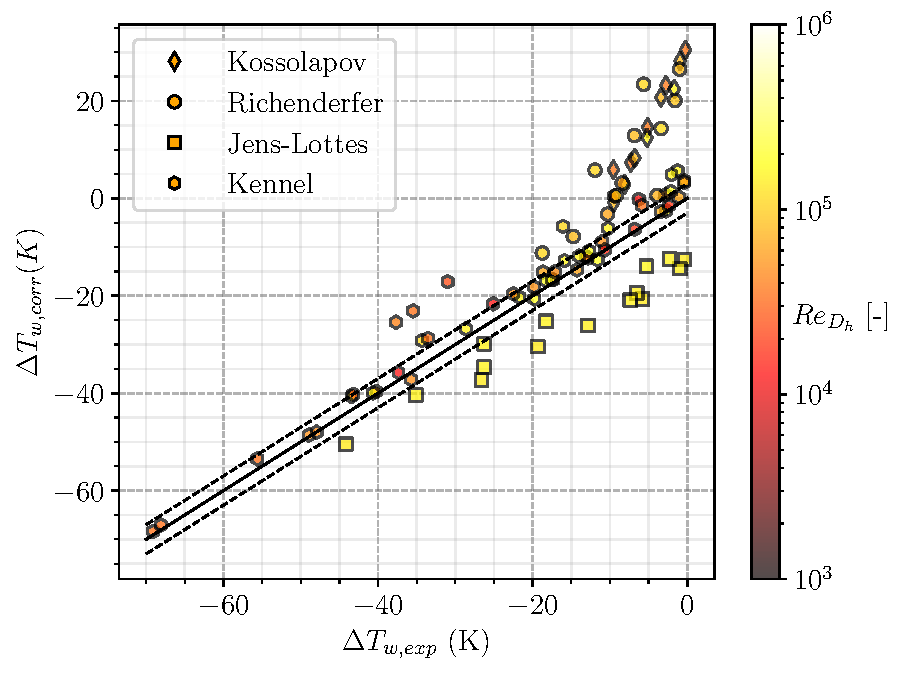
\includegraphics[width=0.45\linewidth]{img/single_phase/comp_dittus.pdf}
\label{fig:dittus_comp}
} 
\subfloat[Gnielinski correlation]{
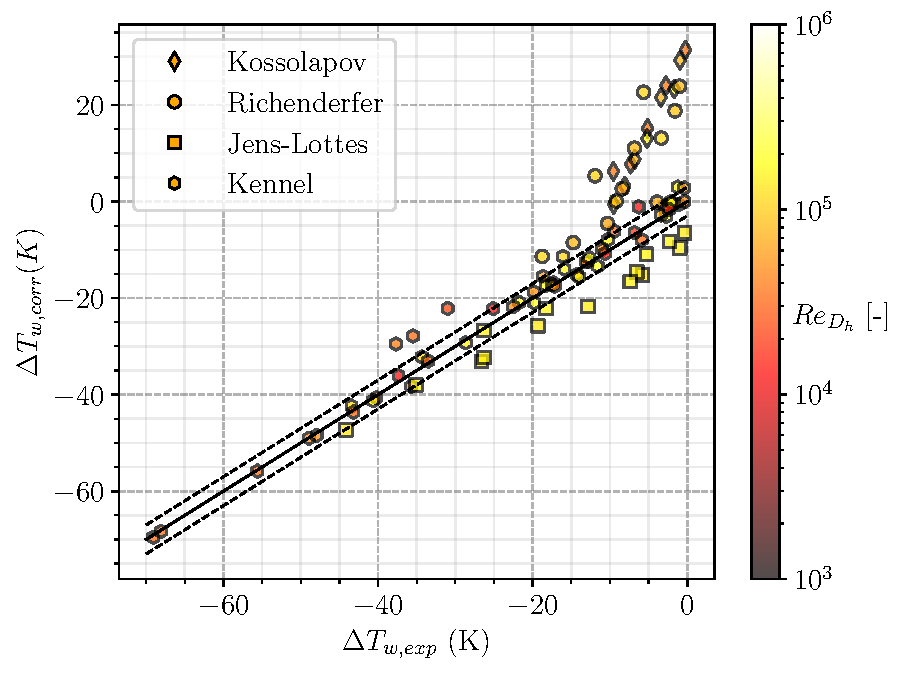
\includegraphics[width=0.45\linewidth]{img/single_phase/comp_gniel.pdf}
\label{fig:gniel_comp}
} 
\caption{Predictive capability of wall temperature by single-phase heat transfer correlations. $\pm 3K$ error bars indicated.}
\label{fig:dittus_gniel_htc}
\end{figure}

The two correlations are of similar efficiency regarding wall temperature predictions over the considered data sets. They both have very good agreement with Kennel data and clear overestimations of $\Delta T_{w}$ on Richenderfer and Kossolapov measurements. The slope difference compared to the parity implies that the correlations are predicting too small Nusselt numbers for those cases. 

Regarding Jens-Lottes data, both model underestimate the wall temperatures, with better results achieved by Gnielinski correlation.

\begin{remark*}{}
We tested different friction factor along with different values of wall roughness in the Gnielinski correlation and observed a negligible impact on the overall results. This allows to stay with a simple formulation for the friction coefficient.
\end{remark*}


The error obtained on Richenderfer and Kossolapov data can be explained by the definition of the HTC computed by Gnielinski correlation. Indeed, Gnielinski correlated a Nusselt number associated to a forced convection coefficient $h_{fc,Gniel}$ in the case of a internal flow with a completely heated wall.

However, only one side of the channel is heated in Richenderfer ans Kossolapov experiments. If $S_{heat}$ denotes this actual heated surface, then Gnielinski correlation estimates the HTC for a surface $4S_{heat}$. With the same imposed total heat power $\Phi_{w}$ and bulk liquid temperature $T_{L}$, we have:

\begin{align}
h_{fc,Gniel} =& \frac{\Phi_{w}}{\parth{T_{w,Gniel}-T_{L}} 4S_{heat}} \\
h_{fc,exp} =& \frac{\Phi_{w}}{\parth{T_{w,exp}-T_{L}} S_{heat}}
\end{align}

Writing $T_{w,Gniel}=T_{w,real}$ then yields:

\begin{equation}
h_{fc,exp}=4h_{fc,Gniel}
\end{equation}

\begin{remark*}{}
This correction can be interpreted as using the thermal diameter instead of the hydraulic diameter, which is 4 times smaller when only one side of the channel is heated.
\end{remark*}

On Figure \ref{fig:ncfd_gniel_corr_htc} we display the predictions of Gnielisnki correlation including this correction by a factor 4 on the HTC for Richenderfer and Kossolapov cases. We also test a $10\%$ reduction on the HTC for Jens-Lottes cases to assess the error made by Gnielinski correlation.

On the same Figure, we also present predictions achieved with the local HTC estimation implemented in NCFD (Eq. \ref{eq:SP_HTC_NCFD}), using a value of $y^{+}=100$. 


\begin{figure}[h!]
\centering
\subfloat[NCFD law]{
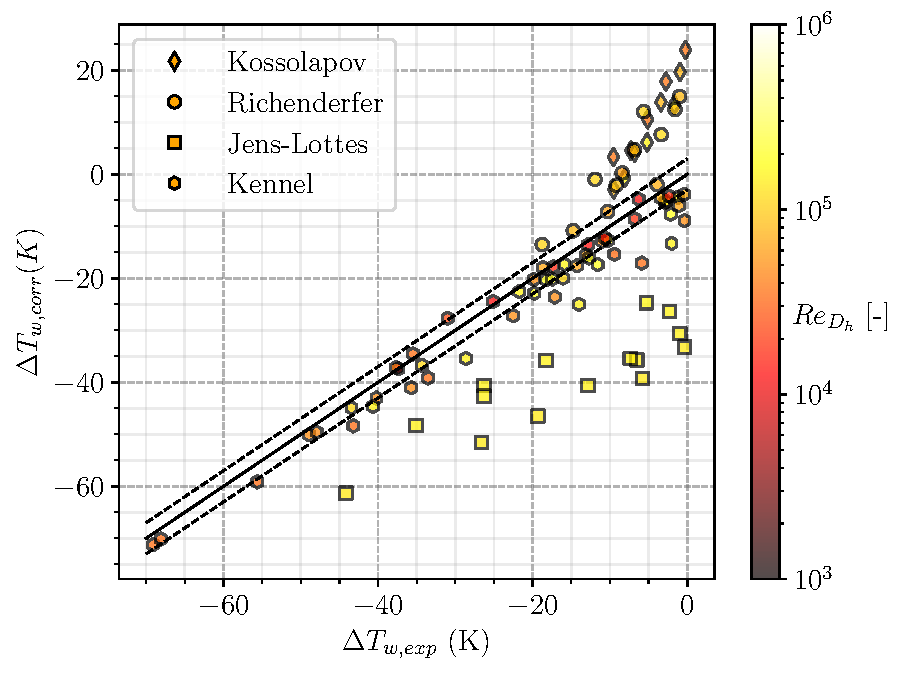
\includegraphics[width=0.45\linewidth]{img/single_phase/comp_ncfd.pdf}
\label{fig:ncfd_comp}
} 
\subfloat[Corrected Gnielinski correlation. We multiply the HTC by 4 on Richenderfer and Kossolapov cases and by 0.9 on Jens-Lotte cases.]{
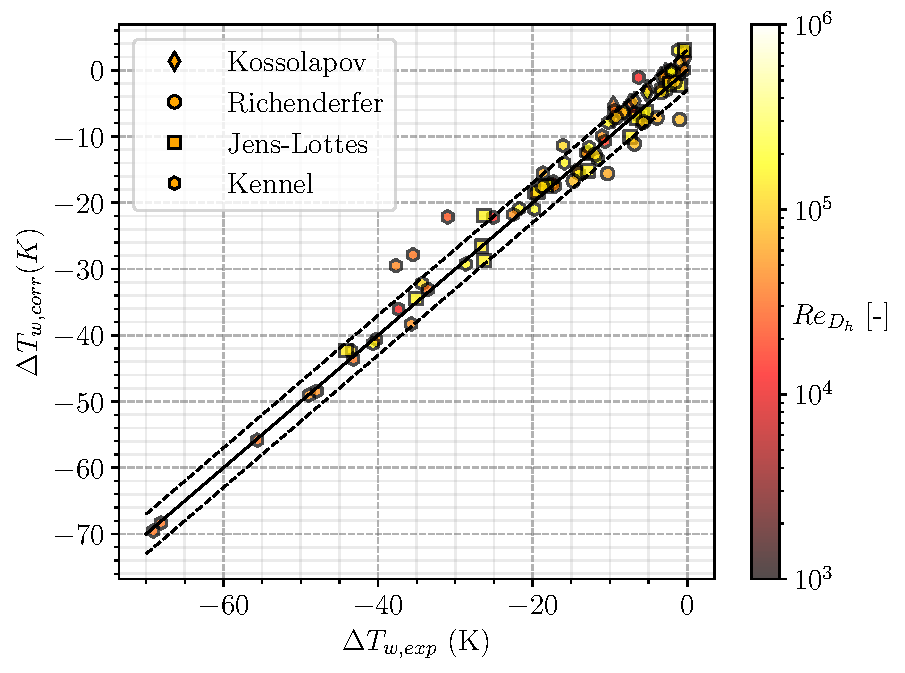
\includegraphics[width=0.45\linewidth]{img/single_phase/comp_gniel_corr.pdf}
\label{fig:gniel_corr_comp}
} 
\caption{Predictive capability of wall temperature by NCFD law and Gnielinski correlation including corrections. $\pm 3K$ error bars indicated.}
\label{fig:ncfd_gniel_corr_htc}
\end{figure}

The NCFD approach yields predictions similar to the 1D correlations (Figure \ref{fig:dittus_gniel_htc}) with larger underestimations on Jens-Lottes measurements. On the other hand, we see that applying a constant correction to the Gnielinski correlation (4 for Kossolapov and Richenderfer cases, 0.9 for Jens-Lottes cases) suffices to yield accurate predictions on the whole range of wall temperature measurements. 

\begin{remark*}{}
The NCFD law was tested without running CFD simulations. The equations were re-written in python to allow its testing outside of the whole code. The use of $y^{+}=100$ as well as the Mac Adams correlation (Eq. \ref{eq:utau_macadams}) for the friction velocity $U_{\tau}$ may induce a difference with the predictions that could be achieved by running a complete CFD computation of the considered cases.
\end{remark*}

The average errors obtained with each model are summed up on Table \ref{tab:error_models_SP_HTC}

\begin{table}[h!]

%\begin{changemargin}{-1cm}{0cm}

\noindent\makebox[\textwidth]{

\scriptsize
\centering
\begin{tabular}{p{25mm}|c c c c c c c c} 
Model & Kossolapov err. [K] & Richenderfer err. [K] & Jens-Lottes err. [K] & Kennel err. [K] \\
\hline
\\

Dittus-Boelter & 19.67 & 15.07 & 10.09 & 3.13 \\
\\

Gnielinski & 20.31 & 14.06 & 6.09 & 1.74 \\
\\

NCFD law & 15.52 & 9.25 & 23.69 & 3.36 \\
\\

Corrected Gnielisnki & 1.34 & 3.08 & 1.57 & 1.74 \\
\\

\hline
\end{tabular}
}
\caption{Average errors achieved by the considered models on each data sets.}
\label{tab:error_models_SP_HTC}
\end{table}


\textbf{Recalling that Gnielinski correlation was also providing good results on the DEBORA cases with R12 (Chapter \ref{chap:debora})further indicates it as a proper choice regarding single-phase HTC estimation in the HFP model.} We will later allow the use of the correction factors when needed to ensure a proper representation of the single-phase part when trying to assess the models associated to boiling.







\section{Nucleation Site Density}
\label{sec:NSD}

The Nucleation Site Density is among the most influencing parameters over the HFP models predictions, particularly regarding wall temperature. Indeed, its value directly controls the density of bubbles generated at the heater and therefore impacts both the boiling ($\phi_{e}$) and quenching ($\phi_{q}$) heat fluxes to the first order. Being able to come up with correct predictions of the NSD is thus critical if one wishes to properly capture the thermal behavior of the boiling surface.

However, the value of $N_{sit}$ is actually influenced by many parameters being either linked to thermal-hydraulics (wall temperature, pressure, operating fluid) or the heater material (roughness, wettability). That is why its value is often estimated through empirical correlations, for which many different expression have been proposed over the years since the end of the XX\textsuperscript{th} century.

\subsection{Existing Correlations}

One of the firstly identified behavior of the NSD was its power dependency with the wall superheat ($N_{sit} \propto {\Delta T_{w}}^{m}$), which is form adopted in the correlation of Lemmert \& Chawla \cite{lemmert_influence_1977} : 

\begin{align}
N_{sit}=\crocht{210\parth{T_{w}-T_{sat}}}^{1.8}
\label{eq:nsit_lemmert}
\end{align}

\begin{remark*}{}
This law is used in the HFP model of Kurul \& Podowski and NEPTUNE\_CFD to compute $N_{sit}$.
\end{remark*}

However, such an expression misses the influence of other parameters such as pressure, which has been proven to be strongly impacting the range of active cavities that can generate bubbles as shown on Figure \ref{fig:nsd_P_koss} and induces a larger bubble density over the heater. 

\begin{figure}[h!]
\centering
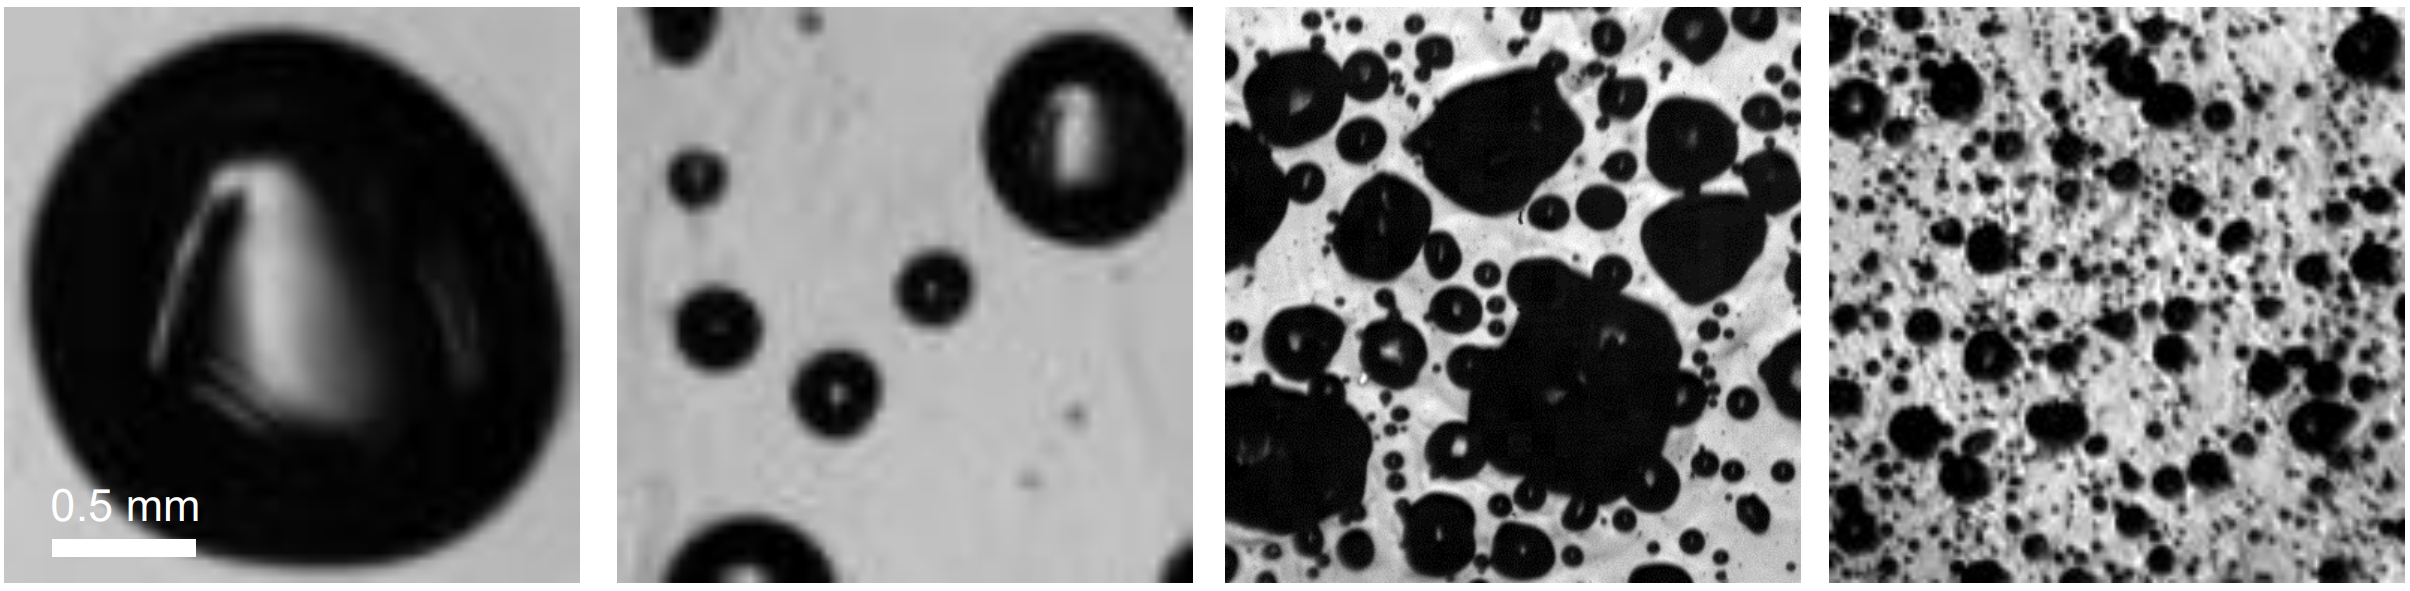
\includegraphics[width=0.7\linewidth]{img/NSD/nsd_press_koss.png}
\caption{HSV Visualization of bubble density at various pressures adapted from Kossolapov \cite{kossolapov_experimental_2021} (left to right: 1.01 bar, 3 bar, 19.8 bar, 75.8 bar). }
\label{fig:nsd_P_koss}
\end{figure}

\npar

Moreover, experimental measurements such as in Borishanskii \cite{borishanskii_heat_1969} showed that the power dependency on the wall superheat changes by increasing both with pressure and the superheat value itself. This was accounted for by Hibiki \& Ishii in 2003 \cite{hibiki_active_2003} who came up with a new correlation that requires an estimation of the minimum activated cavity radius $R_{c}$ : 


\begin{align}
N_{sit} =& N_{0}\parth{1-\exp{-\dfrac{\theta^{2}}{8\mu^{2}} } }\crocht{\exp{ \mathrm{f}\parth{\rho^{+}}\dfrac{\lambda '}{R_{c}} } -1}
\label{eq:nsit_hibiki} \\
%
R_{c} =& \dfrac{2\sigma\parth{1+\dfrac{\rho_{V}}{\rho_{L}}} / P }{\exp{\dfrac{h_{LV} \Delta T_{w}}{R_{g}T_{w}T_{sat}} } -1}\\
%
\mathrm{f}\parth{\rho^{+}} =& -0.01064 + 0.48246\rho^{+} - 0.22712 \rho^{+^{2}} + 0.05468 \rho^{+^{3}}
\end{align}
with $R_{g}$ the perfect gas constant times the molar mass of the fluid,  $N_{0}=4.72\times 10^{5}\ \mathrm{m}^{-2}$, $\mu = 0.722\ \mathrm{rad}$, $\lambda ' = 2.5 \times 10^{-3} \ \mathrm{m}$ and $\rho^{+}=\mathrm{log}_{10}\parth{\dfrac{\rho_{L}-\rho_{V}}{\rho_{V}}}$.


\begin{remark*}{}
This law is used in the HFP model of Gilman \& Baglietto \cite{gilman_self-consistent_2017}.
\end{remark*}

We can note that it also includes the value of the static contact angle $\theta$ which can be used as a parameter to accounts for wall properties, since it is dependent on the wall roughness, wettability and the operating fluid. 

Indeed, a high-wetting material (low values of $\theta$) will allow smaller cavities to be flooded by the surrounding liquid, thus hindering non-condensable gases to be captured inside and become a potentially active nucleation site (Figure \ref{fig:nsd_theta_wet}).

\begin{figure}[h!]
\centering
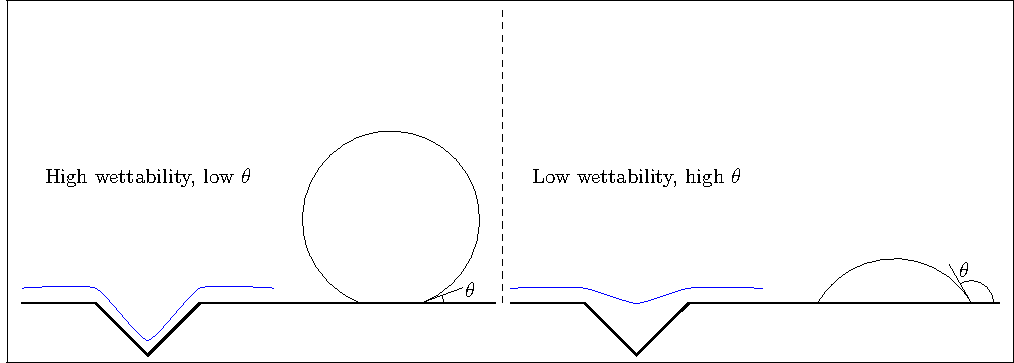
\includegraphics[scale=0.8]{img/NSD/wettability.pdf}
\caption{Sketch of the link between bubble contact angle and wettability / cavity flooding}
\label{fig:nsd_theta_wet}
\end{figure}

This influence of the contact angle on the NSD was confirmed by experimental obervations of Basu \etal \cite{basu_wall_2005} and was also included in a law correlated on their own measurements :

\begin{align}
N_{sit}=&
\begin{dcases}
0.34\crocht{1-\cos{\theta}} {\Delta T_{w}}^{2} & \text{if } \Delta T_{w,ONB}<\Delta T_{w} < 15\ K\\
3.4\times 10^{-5}\crocht{1-\cos{\theta}} {\Delta T_{w}}^{5.3} & \text{if } \Delta T_{w} > 15\ K
\end{dcases}
\label{eq:nsit_basu}
\end{align}

\npar

Similarly, Zhou \etal \cite{zhou_experimental_2020} correlated their measurements, including an influence of the pressure:

\begin{align}
N_{sit} =& N_{0}\parth{1-\cos{\theta}}\crocht{\exp{\mathrm{f}\parth{P} \Delta T_{w} } -1 }
\label{eq:nsit_zhou}\\
&\mathrm{f}\parth{P} = 0.218~\ln{\dfrac{P}{P_{0}}}+0.1907
\end{align}
with $N_{0}=55~395.26\ \mathrm{m}^{-2}$ and $P_{0}=1.01\ \mathrm{bar}$.

\npar

Finally, one of the most recent NSD correlation has been proposed by Li \etal in 2018 \cite{li_new_2018} and validated over a large range of measurements by including a more realistic power law for $\Delta T_{w}$. It avoids the divergence of $N_{sit}$ observed in Hibiki \& Ishii law (Eq. \ref{eq:nsit_hibiki}) when reaching high pressure and superheats. It also includes the impact of pressure and contact angle and its evolution with temperature \eg its decrease close to 0 $\degree$ when approaching the critical temperature \cite{song_temperature_2021}:


\begin{align}
N_{sit} &= N_{0}e^{\mathrm{f}\parth{P}} {\Delta T_{w}}^{A\Delta T_{w} + B} \parth{1- \cos{\theta}}
\label{eq:nsit_li}\\
%
\mathrm{f}\parth{P} &= 26.006 - 3.678 e^{-2P} - 21.907e^{-P / 24.0.65}\\
%
A &= -2\times 10^{-4} P^{2} + 0.0108P + 0.0119\\
%
B &= 0.122P +1.988\\
%
1-\cos{\theta} &= \parth{1-\cos{\theta_{0}}}\parth{\frac{T_{c}-T_{sat}}{T_{c}-T_{0}}}^{\gamma}
\end{align}
with $P$ in MPa, $\theta_{0}$ the contact angle at room temperature $T_{0}$, and default value being for water $\theta_{0}=41.37 \degree$, $T_{c}=374 \degree$C $T_{0}=25\degree$C, $\gamma = 0.719$.

\begin{remark*}{}
We can question the absence of bulk liquid velocity and temperature in the presented law since they should logically influence the nucleation process. However, this impact is rather limited as observed in experimental measurements of Zhou \etal and Kossolapov.
\end{remark*}

\subsection{Comparison with Experimental Measurements}

In order to assess existing NSD correlations and choose the most pertinent to include in a HFP model, we gather NSD measurements from 4 different authors. The different operating conditions of the chosen data sets are gathered on Table \ref{tab:nsit_exp_data}.


\begin{table}[h!]

%\begin{changemargin}{-1cm}{0cm}

\noindent\makebox[\textwidth]{

\scriptsize
\centering
\begin{tabular}{p{20mm}|c c c c c c c c} 
Author & Fluid &  $P$ [bar] & $G_{L}$ [$\debm$] & $\Delta T_{L}$ [K]  & $\Delta T_{w}$ [K] & $\theta_{0}$ [$\degree$] &  $N_{mes}$ [-]\\
\hline
\\

Zhou \cite{zhou_experimental_2020} \newline (2020) & Water & 1.21 - 3.12 & 482.7 - 1930.6 & 8 - 15  & 6.7 - 20.2 & $51$ & 60 \\
\\

Richenderfer \cite{richenderfer} \newline (2018) & Water & 1.01 & 500 - 1000 & 10 & 21.7 - 42.8 & $80$ & 49 \\
\\

Kossolapov \cite{kossolapov_experimental_2021} \newline (2021) & Water & 1.01 - 75.8 & 500 - 2000 & $80$ &10 & 80\degree & 63 & \\
\\

Borishanskii \cite{borishanskii_heat_1969} \newline (1966) & Water & 1.01 - 198 & N.A. & N.A. & 1.75 - 17.3 & $45$ & 132 \\
\\

\hline
\end{tabular}
}

\caption{Nucleation Site Density data in flow boiling}
\label{tab:nsit_exp_data}


\end{table}



We then compare the predictions achieved by the model of Lemmert \& Chawla (Eq. \ref{eq:nsit_lemmert}), Hibiki \& Ishii (Eq. \ref{eq:nsit_hibiki}), Zhou \etal (Eq. \ref{eq:nsit_zhou}) and Li \etal (Eq. \ref{eq:nsit_li}).  The comparison with measurements are presented on Figure \ref{fig:pred_nsit_models}.




\begin{figure}[!h]
\centering
\subfloat[Lemmert \& Chawla model]{
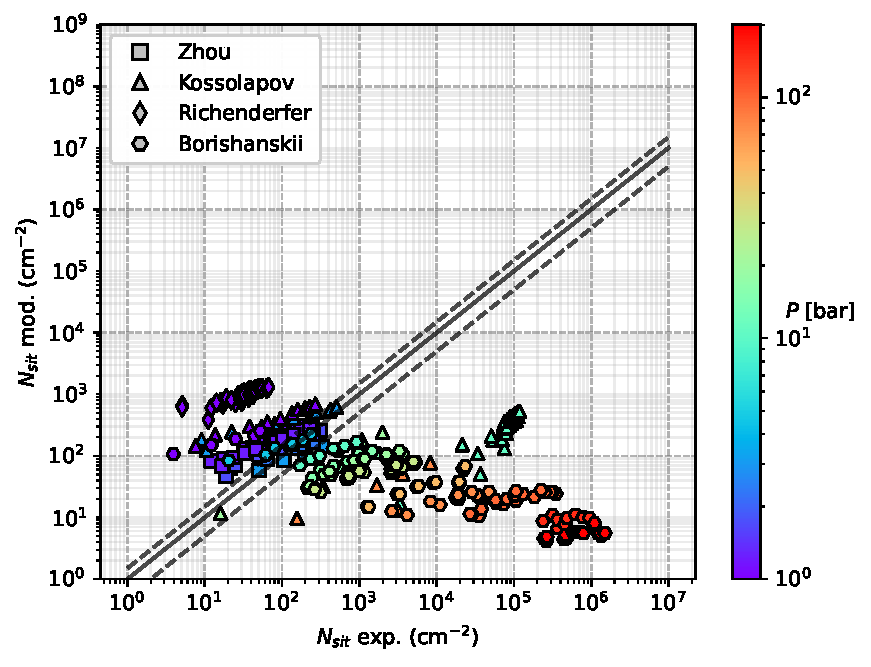
\includegraphics[width=0.45\linewidth]{img/NSD/nsit_LC.pdf}
\label{fig:pred_nsit_lemmert}
} 
\subfloat[Hibiki \& Ishii model]{
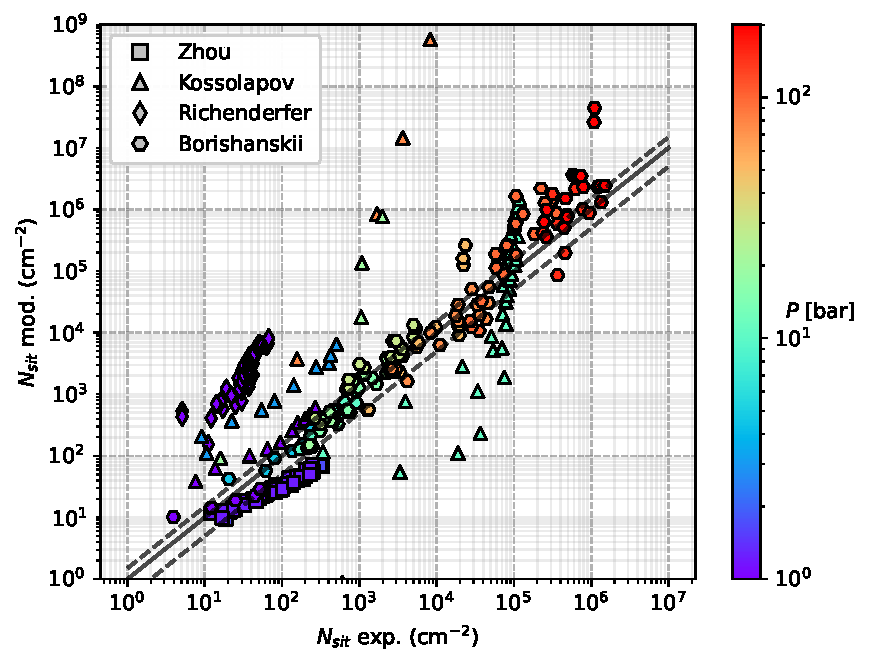
\includegraphics[width=0.45\linewidth]{img/NSD/nsit_HI.pdf}
\label{fig:pred_nsit_hibiki}
}
\\
\subfloat[Zhou \etal model]{
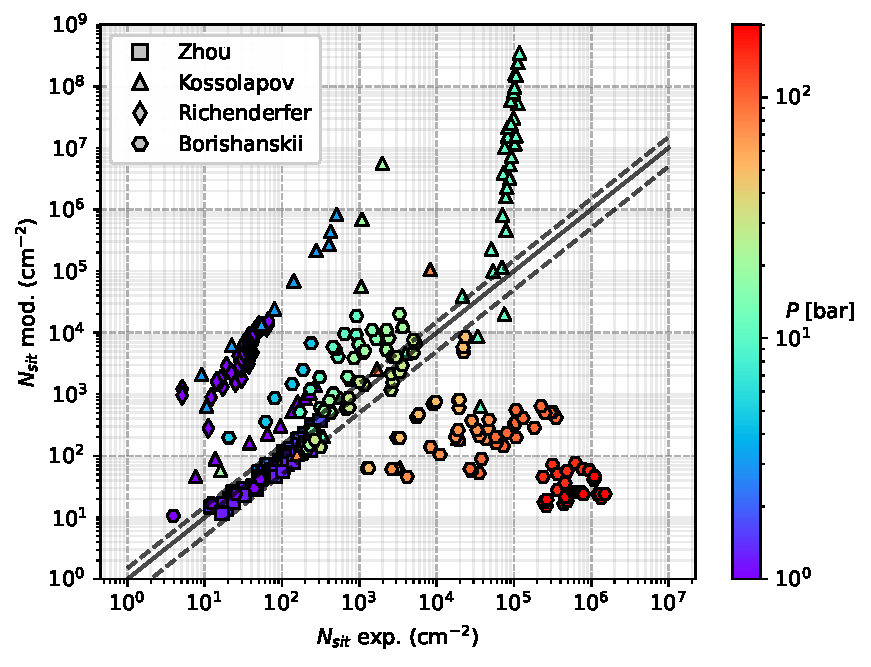
\includegraphics[width=0.45\linewidth]{img/NSD/nsit_Zhou.pdf}
\label{fig:pred_nsit_zhou}
} 
\subfloat[Li \etal model]{
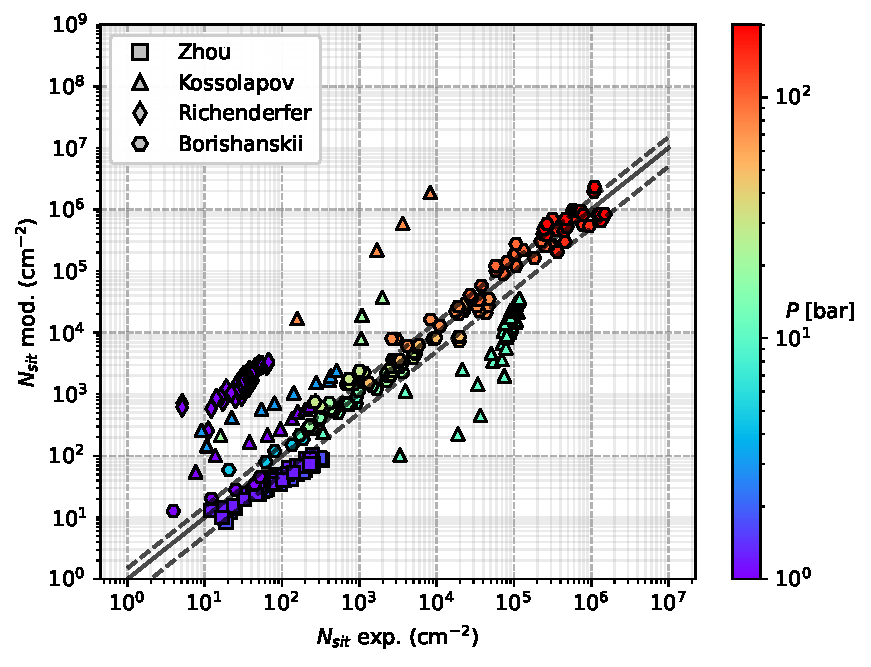
\includegraphics[width=0.45\linewidth]{img/NSD/nsit_Li.pdf}
\label{fig:pred_nsit_li}
}

\caption{Predictions of the chosen models against the experimental data of Table \ref{tab:nsit_exp_data} with $\pm 50\%$ error bars. The contact angles}
\label{fig:pred_nsit_models}
\end{figure}

The Lemmert \& Chawla model appears to fail in predicting the NSD at high pressures. This is a logical drawback of its sole dependence on the wall superheat. More importantly it increasingly underestimates the NSD as pressure increases, which makes it a clearly unsuitable correlation to compute $N_{sit}$ particularly for pressurized flows such as in PWR.

Altough the model of Zhou \etal includes a pressure term, its partial calibration on data covering a low range of pressure may explain the large error observed when compared to higher pressure measurements.

On the contrary, models from Hibiki \& Ishii and Li \etal seem to better reproduce the different trends with flow conditions, especially with pressure. The model from Li \etal achieves better predictions by avoiding to reach unphysically high values of $N_{sit}$ at higher wall superheat compared to Hibiki \& Ishii. This behavior is clear over Kossolapov data at high pressure, where both model lead to overestimations, the strongest discrepancy being associated to Hibiki \& Ishii model.

Overall, the model of Li \etal is the most efficient with an acceptable agreement on most of the data of Borishanskii and Zhou \etal. The measurements of Richenderfer and Kossolapov fail to be precisely reproduced, but it shows a coherent trend and the most limited error when compared to other correlations.

\begin{remark*}{}
The coherency of NSD predictions is hard to ensure since we do not know the exact contact angle and boiling surface morphology in the experiments. This was pointed out by Richenderfer \cite{Richen_phd} who observed significant variation in the NSD value depending on the heater, though keeping the same material (ITO). For instance, this may explain the fact that the NSD measured by Kossolapov at $10.5$ bar is higher than any other pressure on his experiment, leading to both underpredictions and overpredictions of the model of Li \etal depending on the pressure.
\end{remark*}


All things considered, those comparisons show that the Nucleation Site Density remains among the most difficult quantity to evaluate because of its very large variations over experiments, boiling surfaces and flow conditions. Dedicated correlations are hardly precise outside of their establishment databases. However, it remains the best yet only way to compute $N_{sit}$. \textbf{In that regard, the NSD correlation of Li \etal appears to be the most coherent choice.}












\section{Growth time}
\label{sec:growth_time}


As discussed in Section \ref{sec:bub_growth}, the bubble growth can be acceptably modeled as:

\begin{equation}
R\parth{t} = K\Ja_{w} \sqrt{\eta_{L}t}
\end{equation}
with value of $K$ laying roughly between 0.1 and 2 depending on the boiling conditions.

\npar

With a given departure radius $R_{d}$, the bubble growth time until departure from nucleation site $t_{g,d}$ quan be estimated as:

\begin{equation}
t_{g,d} = \parth{\frac{R_{d}}{K \Ja_{w}}}^{2} \frac{1}{\pi \eta_{L}}
\label{eq:tg_dep}
\end{equation}

\begin{note*}{}
If precise estimations of the thermal boundary layer thickness is achievable, the new analytic expression of the bubble growth proposed in Eq. \ref{eq:exp_growth} can be used to express the growth time:

\begin{equation}
t_{g,d} = \crocht{\frac{1}{K_{a}} \ln{1-\sqrt{1-\dfrac{R_{d}}{R_{\infty}}} } }^{2}
\end{equation}
with $K_{a}$ defined as in Eq. \ref{eq:coeff_expgrowth} and $R_{\infty}$ in Eq. \ref{eq:exp_growth}.

\npar
This formulation requires $R_{d} < R_{\infty}$ the equilibrium radius in subcooled pool boiling. Though this condition seems logical physically speaking, it can't be ensured numerically due to the range of values attainable using correlations or other mechanistic models to estimate $R_{d}$.
\end{note*}



\section{Bubble Wait Time}
\label{sec:wait_time}

The wait time between two nucleation events on an active site corresponds to the time needed for the thermal boundary layer to reconstruct after its disruption due to bubble departure from the nucleation site. This process is then intrinsically related to the heater properties and the transient heat transfer with the external liquid flow.



\subsection{Existing Models}

\subsubsection{Analytic Approaches}

Traditional approaches of the wait time estimation rely on the analytic solution to the transient heat transfer in a semi-infinite medium. Assuming that after bubble departure liquid at $T_{L,bulk}$ is displaced towards the wall at $T_{w}$, one can solve the the differential problem with the initial and boundary conditions:

\begin{align}
T_{L}\parth{y,0} &= T_{L,bulk},\ \forall y >0\\
T_{L}\parth{0,0} &= T_{w},\ \forall t > 0
\end{align}

%\begin{align}
%\left. \begin{array}{r} 
%T_{L}\parth{y,0} &= T_{L,bulk},\ \forall y >0\\[1ex]
%T_{L}\parth{0,0} &= T_{L,bulk},\ \forall y >0
%\end{array} \right\} 
%=\pi_b/2
%\end{align}

The solution of this heat transfer problem if given by:


\begin{equation}
T_{L}\parth{y,t} = T_{L,bulk} + \parth{\Delta T_{w} + \Delta T_{L}}\erfc{\frac{y}{2\sqrt{\eta_{L}t}}}
\label{eq:TL_transient}
\end{equation}

For instance, Mikic \& Rohsenow \cite{mikic_bubble_1970} combine this solution with the assumption that a new nucleation will occur over a cavity of radius $R_{c}$ when the vapor temperature reaches:

\begin{equation}
T_{V,nuc} = T_{sat} + \frac{2\sigma T_{sat} \parth{\dfrac{1}{\rho_{V}} - \dfrac{1}{\rho_{L}} }}{R_{c}h_{LV}}
\label{eq:TVnuc_Mikic} 
\end{equation} 

The wait time is then assumed to be the time needed for the transient temperature field to reach $T_{V,nuc}$ at height $y=R_{c}$ \ie $T_{L}\parth{R_{c},t_{w}}=T_{V,nuc}$. Combining Eq. \ref{eq:TL_transient} and \ref{eq:TVnuc_Mikic} allow to write:

\begin{align}
t_{w} &= \frac{1}{4\eta_{L}} \crocht{ \frac{R_{c}}{\erfcrec{ \dfrac{\Delta T_{L}}{\Delta T_{L} + \Delta T_{w}} + T_{sat} \parth{\dfrac{1}{\rho_{V}} - \dfrac{1}{\rho_{L}}}\dfrac{2\sigma }{ \parth{\Delta T_{w} + \Delta T_{L}}h_{LV}R_{c} } } } }^{2}\\
%
& \approx \frac{1}{\pi \eta_{L}}\crocht{\frac{ \parth{\Delta T_{w} + \Delta T_{L}}R_{c} }{\Delta T_{w} - T_{sat} \parth{\dfrac{1}{\rho_{V}} - \dfrac{1}{\rho_{L}}}\dfrac{2\sigma  }{R_{c} h_{LV}} } }^{2}
\label{eq:twait_mikic}
\end{align}

Using the same approach, Han \& Griffith \cite{han_griffith_tw} use the same expression of the transient liquid temperature field but consider $T_{L}\parth{\dfrac{3}{2}R_{c},t_{w}}=T_{V,nuc}$, which yields a wait time that is $\dfrac{9}{4}$ times Eq. \ref{eq:twait_mikic}.

\npar

Later, Yeoh \etal followed a similar derivation to propose an expression of the wait time that accounts for the contact angle value:

\begin{align}
t_{w} &= \frac{1}{\pi \eta_{L}}\crocht{ \frac{\parth{\Delta T_{L} + \Delta T_{w}} C_{1} R_{c}}{\Delta T_{w} - \dfrac{2\sigma T_{sat}}{C_{2}\rho_{V}h_{LV}R_{c}}}  }^{2}
\label{eq:twait_yeoh}\\
%
C_{1} &= \frac{1 + \cos{\theta} }{\sin{\theta}}\ ;\ C_{2} = \frac{1}{\sin{\theta}}
\end{align}

\npar

All those analytical approaches present one pivotal parameter: the activated cavity radius $R_{c}$. It is a very complicated parameter to evaluate since it can vary by decades depending on the flow conditions and the boiling surface morphology. 

\npar

Among existing expressions of $R_{c}$, we have:

\begin{align}
R_{c} &= \frac{2\sigma T_{sat}}{\rho_{V}h_{LV}\Delta T_{w}},\ \text{used by Han \& Griffith}
\label{eq:rc_han}\\
%
R_{c} &= \sqrt{\dfrac{1}{C_{1}C_{2}} \dfrac{2 \sigma T_{sat} \lambda_{L}}{\rho_{V}h_{LV}\phi_{w}}}, \ \text{used by Yeoh \etal}
\label{eq:rc_yeoh}\\
%
R_{c} &= \frac{2\sigma\parth{1+ \dfrac{\rho_{V}}{\rho_{L}} } / P}{\exp{h_{LV} \dfrac{\Delta T_{w}}{R_{g}T_{w}T_{sat}} }}, \ \text{used by Hibiki \& Ishii}
\label{eq:rc_hibiki}
\end{align}

\begin{remark*}{}
Those analytic expressions do not include the influence of an external liquid velocity, which could have an impact over the wait time since it modifies the hydrodynamics controlling the reconstruction of the thermal boundary layer. In particular, turbulent flows could induce a larger mixing effect between the bulk and the wall thus increasing the time needed to reach sufficient superheat to allow a new nucleation to occur.
\end{remark*}



\subsubsection{Empirical Correlations}

Alternatively, other authors considered the wait time estimation through empirical correlations based on data-fitting on given measurements. For instance, Basu \etal \cite{basu_wall_2005} proposed:

\begin{equation}
t_{w} = 139.1\Delta {T_{w}}^{-4.1}
\end{equation}
based on low pressure and low liquid velocity experiments.


\npar

More recently, Kommajosyula \cite{kommajosyula_development_2020} included the effect of the liquid subcooling through the liquid Jakob number $\Ja_{L}$ as:
\begin{equation}
t_{w} = 0.061\frac{{\Ja_{L}}^{0.63}}{\Delta T_{w}}
\end{equation}

\begin{remark*}
This expression will yield $t_{w}=0$ for saturated boiling conditions, which is hardly reasonable since a non-zero wait time exists between two nucleation events even at saturation \cite{gerardi_ijhmt_2010}.
\end{remark*}



\subsection{Experimental Measurements}

To try to assess the proposed expressions of the bubble wait time, we rely on some experimental measurements available in the literature from Basu \etal \cite{basu_wall_2005}, Richenderfer \cite{richenderfer_phd} and Kossolapov \cite{kossolapov_experimental_2021}. The boiling conditions of the data are summed up on Table \ref{tab:tw_exp_data}.

\begin{table}[h!]

%\begin{changemargin}{-1cm}{0cm}

\noindent\makebox[\textwidth]{

\scriptsize
\centering
\begin{tabular}{p{20mm}|c c c c c c c} 
Author & Fluid & $P$ [bar] & $G_{L}$ [$\debm$] & $\Delta T_{L}$ [K] & $\phi_{w}$ [MW/m\up{2}] & $\Delta T_{w}$ [K] & $t_{w}$ [ms] ($N_{mes}$)\\
\hline
\\

Basu \etal \cite{basu_wall_2005} \newline (2005) & Water & 1.01 & 346.0 & 8.35 - 46.5 & N.A. & 9.83 - 17.5 & 0.797 - 13.3 (19) \\
\\

Richenderfer \cite{richenderfer_phd} \newline (2018) & Water & 1 - 2 & 1000 - 2000 & 5 - 20 & 0.74 - 7.13 & N.A. & 0.914 - 6.02 (259) \\
\\

Kossolapov \cite{kossolapov_experimental_2021} \newline (2021) & Water & 10.5 & 500 - 2000 & 10 & N.A. & 0.12 - 25.9 & 6.13 - 85.9 (33) \\
\\
\hline
\end{tabular}
}

\caption{Bubble wait time data in vertical flow boiling. Wall superheat values for Richenderfer data are estimated using Frost \& Dzakowic correlation (Eq. \ref{eq:frost}).}
\label{tab:tw_exp_data}

%\end{changemargin}

\end{table}

The experimental data are all using water as working fluid. We can see at first glance that values measured by Kossolapov are nearly a decade larger compared to the other experiments. This may be an effect of pressure due to:

\begin{itemize}
\item The bubbles that are smaller and depart nearly right after nucleation, leaving wait time as the main part of the nucleation cycle ;
\item The wall Jakob number values that are smaller ;
\item The heterogeneity in nucleation sites behavior (their number increasing with pressure), with sites exhibiting very large wait time due to their very low nucleation frequency versus very active sites that contributes much more to the overall nucleation. Averaging over those events as done by Kossolapov \cite{kossolapov_experimental_2021} may result in a large wait time.
\end{itemize}


\begin{figure}[!h]
\centering
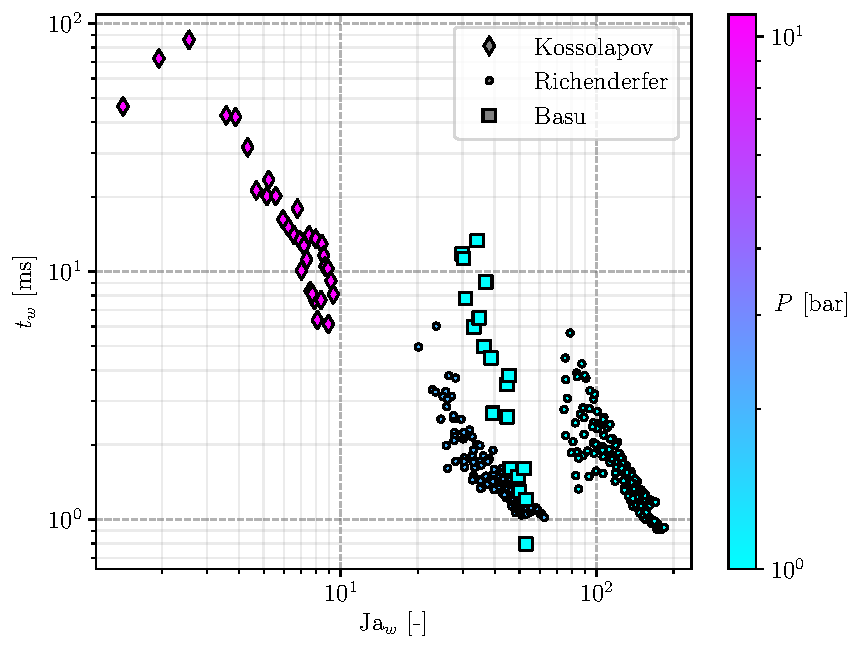
\includegraphics[width=0.6\linewidth]{img/tw/Jaw_tw.pdf}
\caption{Evolution of the wait time values with the wall Jakob number.}
\label{fig:tw_Jaw}
\end{figure}

On Figure \ref{fig:tw_Jaw}, we show the evolution of the measures wait times with the wall Jakob number. We can see that the lower values of Jakob number actually correspond to lower wait times, which seem to confirm the previous assumptions.

\npar

Moreover, we see that there is a steep decrease of the wait time with $\Ja_{w}$. The slope however changes depending on the data set, which would logically depend on the heater thermal properties as well as on the operating fluid. It seems that the slope followed by Kossolapov data at 10 bar seem to align with that of Richenderfer data at 2 bar, which would exhibit a sort of coherency between those two data sets.

On the contrary, values at 1 bar from Basu do not clearly match with Richenderfer data at 1 bar.

\npar

The data sets from Kossolapov and Richenderfer also give the associated frequency to each wait time measurement. This allows to plot the product $t_{w} \times f$ to evaluate the proportion of the nucleation cycle occupied by wait time. The value of $t_{w} \times f$ would physically be expected to tend to $1$ when $\Delta T_{w} \to 0$ (highly reduced nucleation) and to $0$ when $\Delta T_{w} \to \infty$ due to the intense nucleation and increased transient heat transfer under the high temperature gradient between the wall and the fluid. Experimental values are plotted on Figure \ref{fig:twf_Jawred} versus the reduced Jakob number values to regroup the values by excluding the influence of the density ratio $\rho_{L}/\rho_{V}$.



\begin{figure}[!h]
\centering
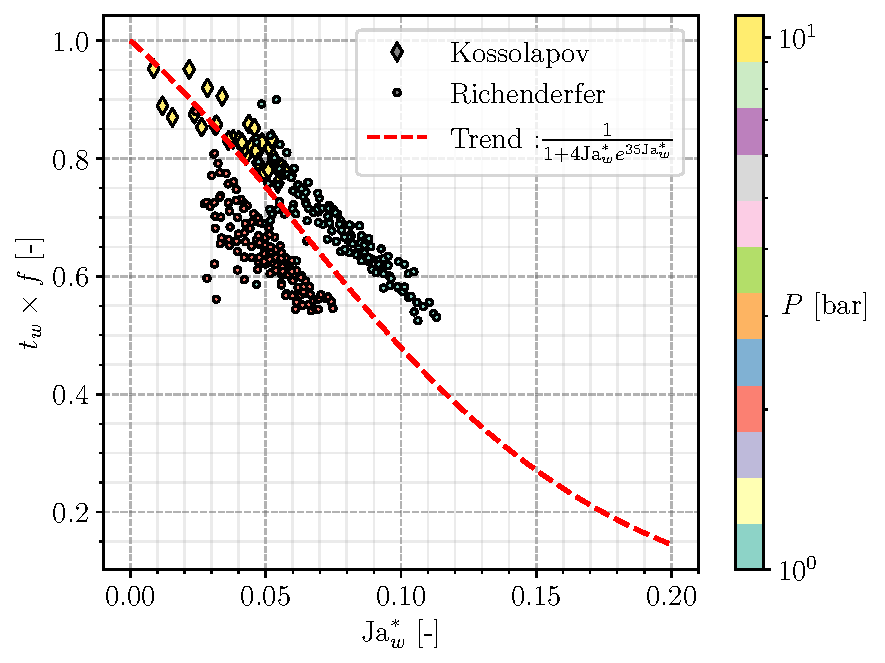
\includegraphics[width=0.6\linewidth]{img/tw/Jawred_twf.pdf}
\caption{Evolution of the product $t_{w} \times f$ with the reduced Jakob number.}% Trend line is of the form $t_{w} f = \dfrac{1}{1+A\Ja_{w}^{*}\exp{B\Ja_{w}^{*}}}$.}
\label{fig:twf_Jawred}
\end{figure}

We can see that for lower values of $\Ja_{w}^{*}$, the product $t_{w} \times f$ starts to tend to $1$. For higher values, a linear decrease seem to be the general trend of the measurements. However, it can't decrease linearly forever, which is why the trend on Figure \ref{fig:twf_Jawred} extrapolated to higher values of $\Ja_{w}^{*}$ looks like a sigmoid in order to approach zero for large superheats. Nevertheless, we clearly lack of measurements at larger values of $\Ja_{w}^{*}$ to confirm this supposed trend.

\begin{remark*}{}
The range of values attained by the product $t_{w} \times f$ can vary from 1 down to 0.5 on the chosen experimental data. This clearly shows that the relation between the wait time and the growth time is not straightforward as assumed in some works who neglects the growth time or suppose a constant relationship such as $t_{w}=3t_{g}$\cite{han_griffith}.

\npar
Moreover the boiling conditions range covered by the data are not that exhaustive, leaving room for even larger ranges of $t_{w} \times f$ with different fluids and heater material for instance.
\end{remark*}

\subsection{Evaluation of the Models}

Using the data of Table \ref{tab:tw_exp_data} to evaluate the different approaches presented above, we obtain the results presented on Figures \ref{fig:tw_pred_correl} and \ref{fig:tw_pred_anal}.


\begin{figure}
\centering
\subfloat[Basu \etal correlation]{
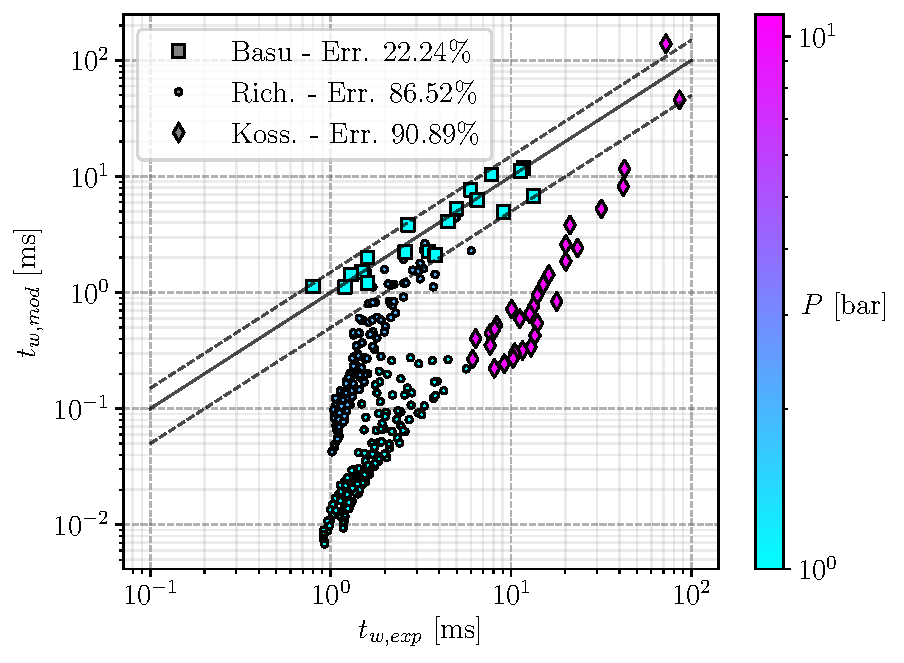
\includegraphics[width=0.5\linewidth]{img/tw/tw_Basu.pdf}
}
\subfloat[Kommajosyula correlation]{
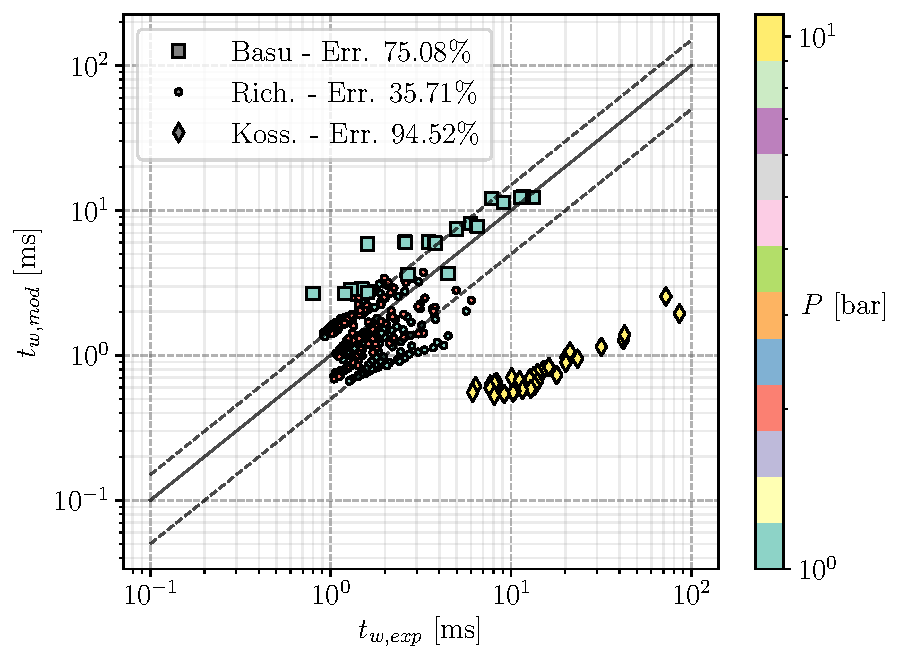
\includegraphics[width=0.5\linewidth]{img/tw/tw_Komma.pdf}
}
\caption{Predictions using the correlations. $\pm 50\%$ dashed lines are represented.}
\label{fig:tw_pred_correl}
\end{figure}

\npar
The correlation of Basu \etal naturally performs well on their own data but largely underestimates the wait time for Richenderfer and Kossolapov data. Kommajosyula's formulation produces better results on the low pressure cases, particularly on Richenderfer cases. However, it fails to capture the increase in $t_{w}$ for Kossolapov data and largely underestimates them.


\begin{figure}
\centering
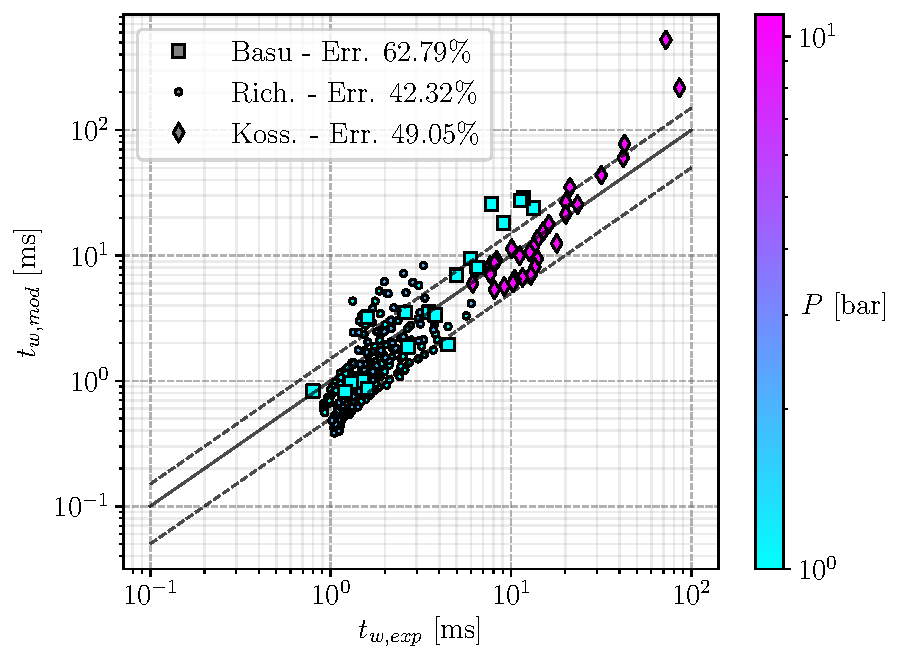
\includegraphics[width=0.5\linewidth]{img/tw/twYeoh_RcHan.pdf}
\caption{Yeoh \etal formulation of $t_{w}$ with Han \& Griffith cavity radius. $\pm 50\%$ dashed lines are represented.}
\label{fig:tw_pred_anal}
\end{figure}

\npar
When testing the analytic formulations of the wait time, we tested different combinations of ($t_{w}$, $R_{c}$) expressions. Overall, we saw that the results were strongly dependent on the value of the cavity radius with values that can change by decades depending on the chosen formulation.

\npar
At last, it appeared that choosing the Yeoh \etal expression of $t_{w}$ (Eq. \ref{eq:twait_yeoh}) along with the cavity radius of Han \& Griffith (Eq. \ref{eq:rc_han}) resulted in good results in average over the three chosen datasets. As we can see on Figure \ref{fig:tw_pred_anal}, it produces overall better results compared to the correlation. Moreover, we used contact angle values that were representative of each experimental conditions according to each author:

\begin{itemize}
\item $\theta = 31 \degree$ for Basu \etal data \cite{basu_wall_2005-1} ;
\item $\theta = 72 \degree$ for Richenderfer data \cite{richenderfer_phd};
\item $\theta = 80 \degree$ for Kossolapov data \cite{kossolapov_experimental_2021}.
\end{itemize} 

The fact that the analytic expression is able to correctly predict the large range of $t_{w}$ values from the different experiments is encouraging since it is based on a physical approach contrary to correlations which mainly relies on data-fitting.

\textbf{To conclude, it seems appropriate to use the wait time formulation of Yeoh \etal along with expressing cavity radius using Han \& Griffith estimation.}






\section{Bubble Sliding Length}

\section{Single Bubble Quenching Area}


\label{sec:quench_area}

When computing the quenching heat flux, we need to provide the total wall area visited by a single bubble $A_{q,1b}$ that will undergo quenching.

In wall boiling model that do not consider bubble sliding \cite{kurul_podowski, guelfi_neptune_2007, shaver_podowski} the impacted area at bubble lift-off is often considered as :

\begin{equation}
A_{q,1b} = F_{A} \pi R_{lo}^{2}
\end{equation} 
with $F_{A}$ being an enhancement factor that accounts for the the possibility that the bubble will induce quenching over a surface larger than its projected area.



\begin{align}
A_{q,1b} = &
\begin{dcases}
\pi R_{lo}^{2} & \text{if } l_{sl}\leq R_{lo}-R_{d} \\
%
\frac{1}{2}\pi R_{d}^{2} + l_{sl}\parth{R_{d}+R_{lo}} + \frac{1}{2}\pi R_{lo}^{2} & \text{if } l_{sl} \geq R_{lo}+R_{d}
%
\end{dcases}
\end{align}

Which can be re-expressed by defining ${l_{sl}}^{*}=\dfrac{l_{sl}}{R_{lo}}$ and ${A_{q,1b}}^{*}=\dfrac{A_{q,1b}}{\pi R_{lo}^{2}}$

\begin{align}
{A_{q,1b}}^{*} = &
\begin{dcases}
1 & \text{if } {l_{sl}}^{*}\leq 1- \frac{R_{d}}{R_{lo}} \\
%
\frac{1}{2}\parth{1+\parth{\frac{R_{d}}{R_{lo}}}^{2} } + \frac{{l_{sl}}^{*}}{\pi}\parth{1+\frac{R_{d}}{R_{lo}}} & \text{if } {l_{sl}}^{*} \geq 1 + \frac{R_{d}}{R_{lo}}
\end{dcases}
\end{align}
and we linearly interpolate those two expressions for the region where $1-\dfrac{R_{d}}{R_{lo}}\geq {l_{sl}}^{*} \geq 1+\dfrac{R_{d}}{R_{lo}}$.





\section{Considerations on Bubble Interactions and Nucleation Sites Deactivation}

\subsection{Nucleation Site Distribution}

NSD correlations actually estimate the total number of sites where bubbles can nucleate on a surface. However, experimental observations showed that nucleation sites exhibit largely heterogeneous behaviors. For instance, Figure \ref{fig:sites_f_koss} shows experimental observations from Kossolapov \cite{kossolapov_experimental_2021} that demonstrate the variety of nucleation frequency measured for each site on a boiling surface.

\begin{figure}[!h]
\centering
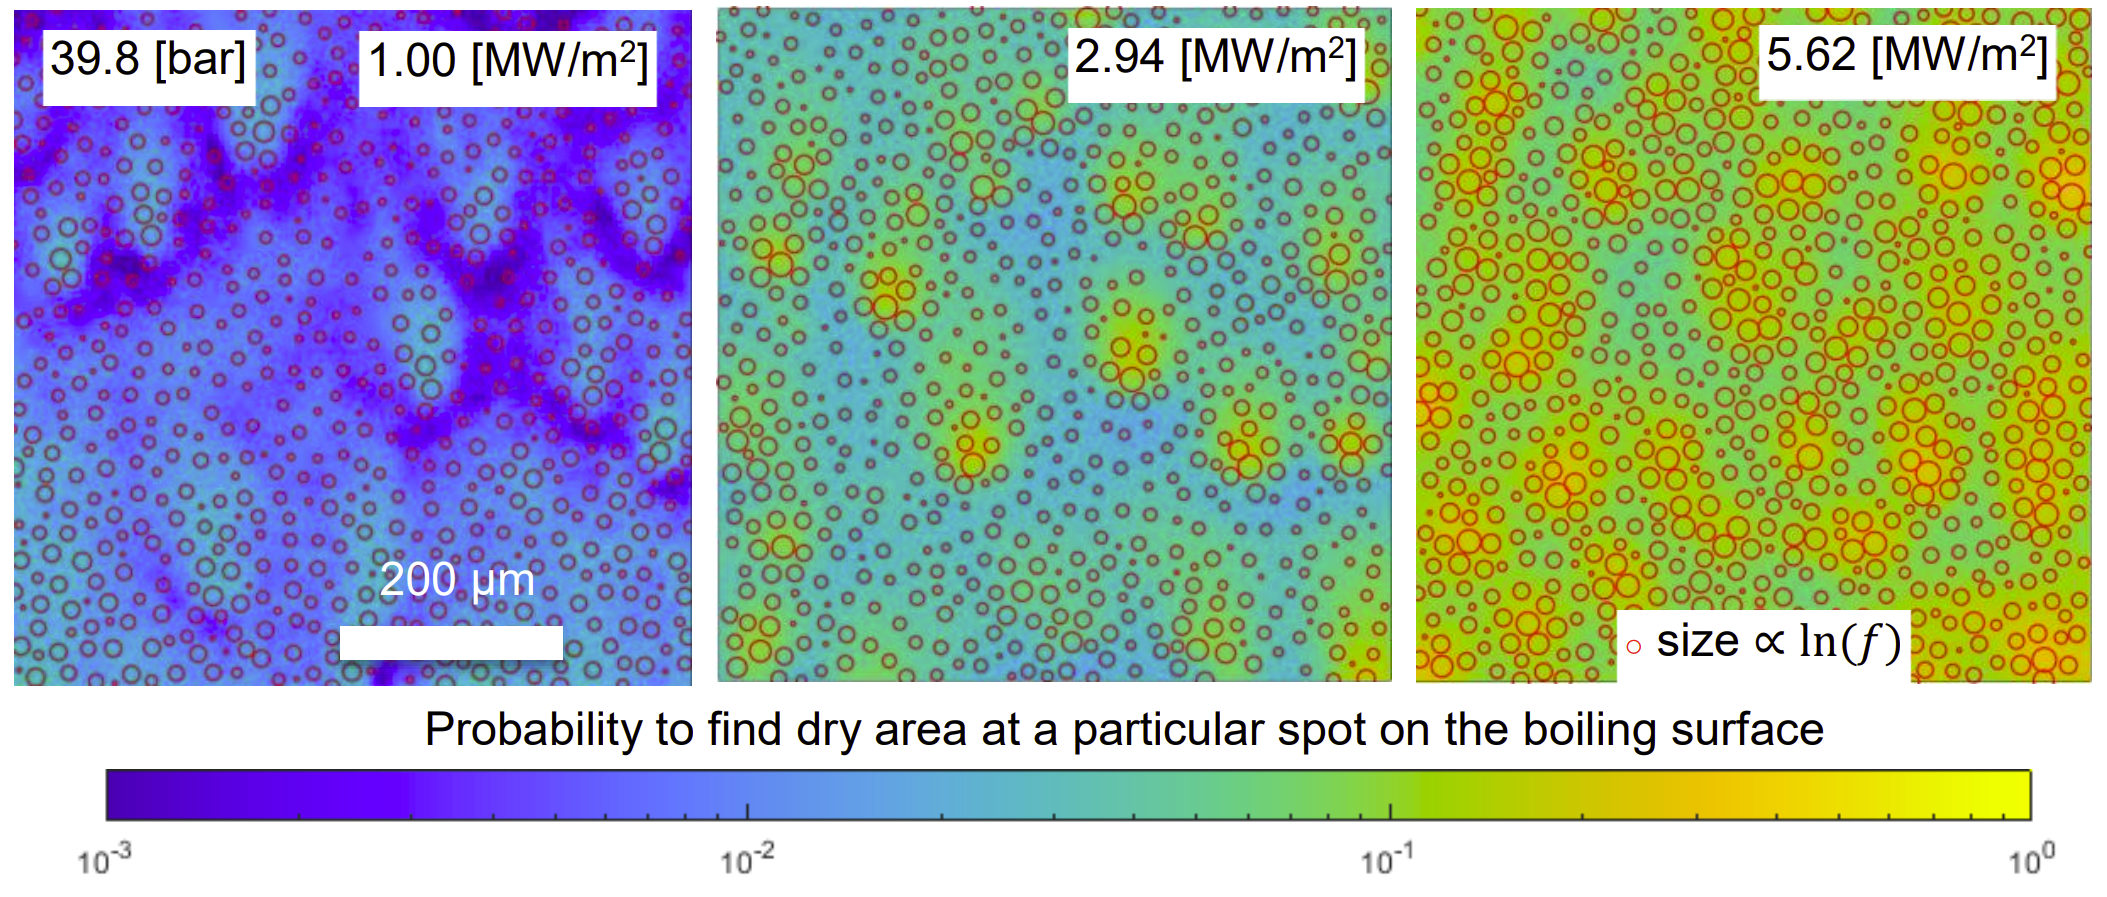
\includegraphics[width=0.9\linewidth]{img/site_interaction/site_f_kossolapov.PNG}
\caption{Nucleation site distribution with associated nucleation frequency, by and adapted from Kossolapov \cite{kossolapov_experimental_2021}.}
\label{fig:sites_f_koss}
\end{figure}

\npar

This large difference in nucleation frequency between the different sites indicates that a minority of sites contribute to most of the total phase change process. Those differences may originate from different interactions such as:

\begin{itemize}
\item Thermal deactivation: a bubble nucleating at a site gathers the energy in the wall to use it for phase change, which in turns locally decreases the temperature and will hinder nucleation to occur at neighboring sites.
\item Static deactivation: given a number of active sites, distributing a number of bubbles of radius $R_{d}$ over them can lead to overlapping that can not geometrically be accommodated on the wall. This effect was notably considered by Gilman \& Baglietto \cite{gilman_self-consistent_2017}.
\item Sliding deactivation: if a bubble slides and swipes a given area, sites laying on its path may experience quenching even before holding a nucleating bubble. This consequently will impact their nucleation frequency and may lead to partial deactivation under the sliding effect.
\end{itemize} 


In order to consider such interactions between nucleation sites, we need to know their spatial distribution over the boiling surface. Usual approaches considered that the nucleation sites followed an homogeneous spatial Poisson process \ie the probability of finding a site in an area $A$ only depends on the value of $A$ and not on its location over the boiling surface.

\npar
This has been supported by different experimental observations such as those of Gaertner \cite{gaertner_1960} or Sultan \cite{sultan_1978} for pool boiling who found an agreement between site distribution and Poisson process by studying sites populations in subdivisions of the boiling surface. It was also confirmed for flow boiling by Del Valle \& Kenning \cite{kenning_boiling} who observed site distribution at different heat fluxes. However, they noticed that the increase in nucleation site with the heat flux did not come from an additive effect of new sites since some active sites at low heat fluxes became inactive at higher heat fluxes before sometimes reactivating later (see Figure \ref{fig:kenning_boiling_inter}. This further highlights that the interactions and deactivation processes originate from complex physics that simultaneously include wall morphology and thermal behavior, external flow influence and bubble presence. 

\npar

More recent observations also show a random distribution of the sites such as in Zhou \etal \cite{zhou_experimental_2020-1} (Figure \ref{fig:zhou_sites}).

\begin{figure}[!h]
\centering

\subfloat[Nucleation site distribution in flow boiling from Del Valle \& Kenning \cite{del_valle_subcooled_1985}. Black triangles circled in red represent sites that deactivate when the heat flux exceeds 70\% of the CHF. ]{
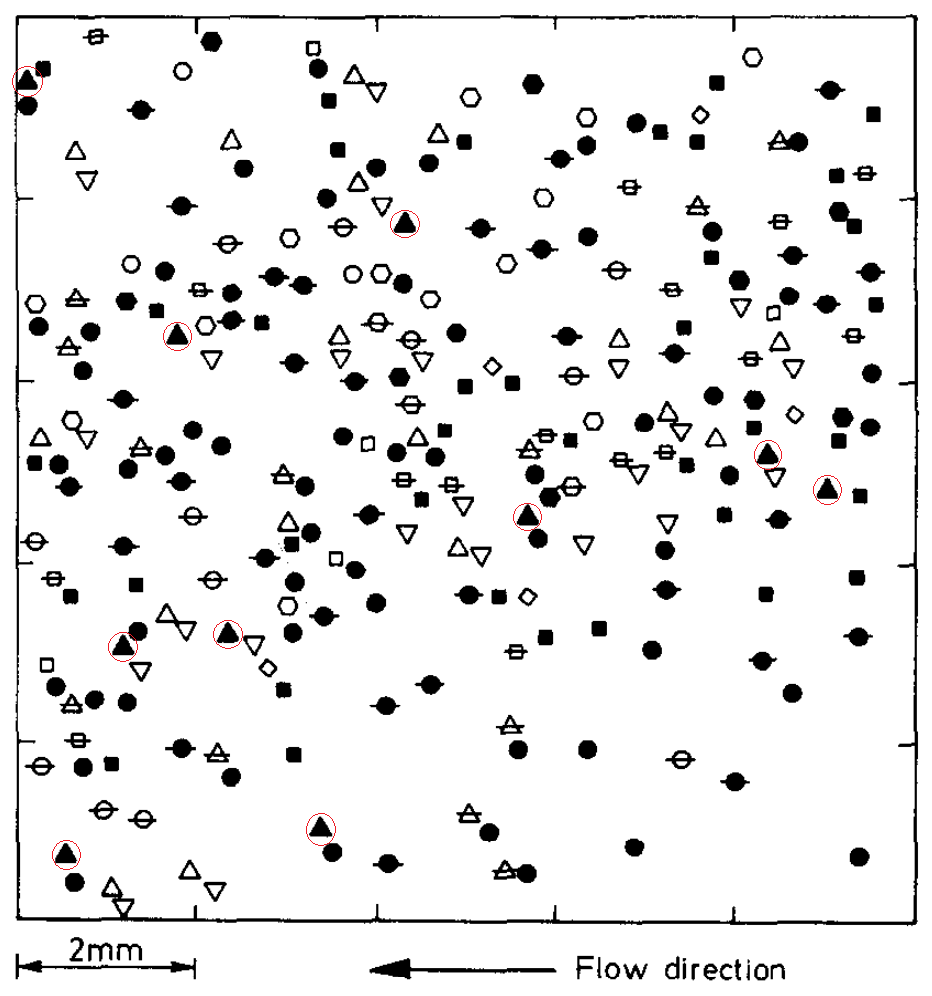
\includegraphics[width=0.5\linewidth]{img/site_interaction/sites_kenning_red.PNG}
\label{fig:kenning_boiling_inter}
}
\\
\subfloat[Nucleation site distribution at 3 bar by and adapted from Zhou \etal \cite{zhou_experimental_2020}.]{
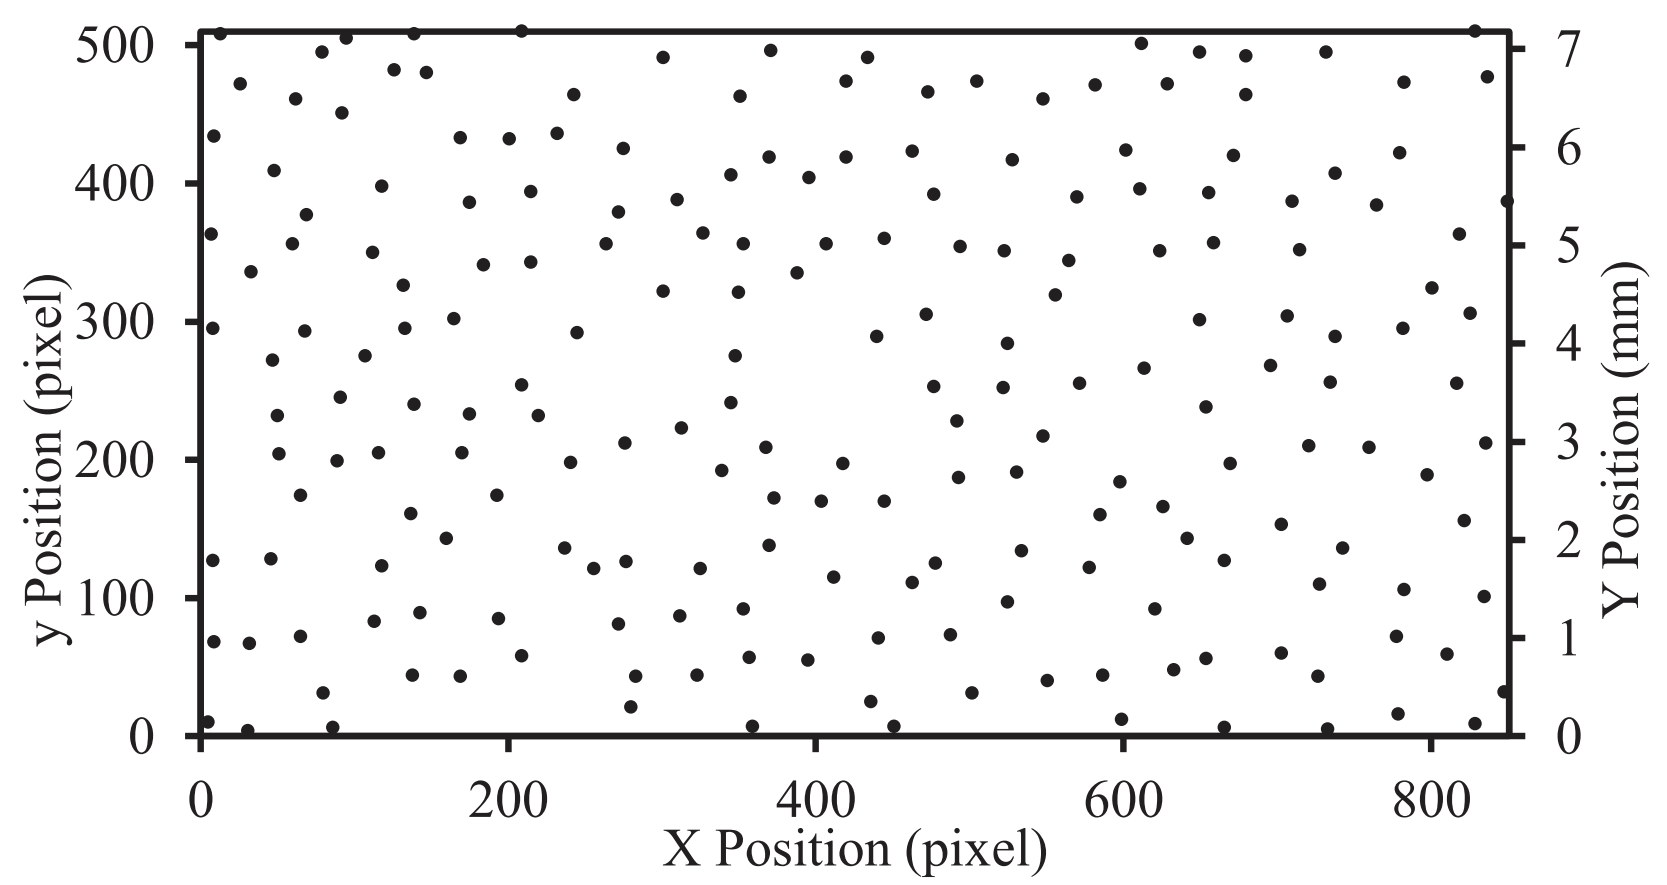
\includegraphics[width=0.7\linewidth]{img/site_interaction/sites_zhou.PNG}
\label{fig:zhou_sites}
}

\caption{Examples of exprimental nucleation sites distribution in flow boiling.}
\label{fig:sites_distribution}
\end{figure}

\npar

Considering an homogeneous spatial (two-dimensional) Poisson process with an event density (\ie average number of events per unit of area) $\delta$, then the probability that the number of event $N$ in an area $A$ is equal to $n \ in \mathbb{N}$ is \cite{Daley_vere-jones_point_processes}:

\begin{equation}
\mathcal{P}\parth{N\parth{A}=n}=\frac{\parth{\lambda A}^{n}}{n!}e^{-\lambda A}
\label{eq:poisson_proba}
\end{equation}

Then, one can express the probability density function of the nearest-neighbor, depending on the distance $r$ between two events as:

\begin{align}
f\parth{r}=2\lambda \pi r e^{-\lambda \pi r^{2}}
\label{eq:poisson_distribution}
\end{align} 


This special case of Poisson point-processes is also called "Complete Spatial Randomness".


\begin{remark*}{}
Although observations of the boiling surface presented random distributions of sites close to a Poisson process, Del Valle \& Kenning \cite{del_valle_subcooled_1985} found that the measured nearest-neighbor distance distribution was deviating from Eq. \ref{eq:poisson_distribution} for low values of $r$.
\end{remark*}

Eq. \ref{eq:poisson_distribution} allows to compute the average distance $s$ betwen two events:

\begin{equation}
s = \int_{0}^{+\infty} r f\parth{r}\mathrm{d}r  = 2 \frac{\sqrt{\pi}}{4\sqrt{\lambda \pi}} = \frac{1}{2\sqrt{\lambda}}
\end{equation}


\npar

From those mathematical expressions, we can then model different type of interactions between sites by choosing proper event densities $\lambda$. Further subsections propose treatments of a few of them.


%\npar
%
%In order to physically take into account this effect, Gilman considered a statistical approach, by assuming that nucleation site are randomly distributed over the heater surface (Complete Spatial Randomness). Then, considering that a nucleation site located under a bubble will be deactivated, one can express the number of sites actually contributing to bubble nucleation $N_{sit,a}$ as :
%
%
%\begin{align}
%N_{sit,a}=\parth{1-\mathcal{P}}N_{sit},\ \text{with}\ \mathcal{P}=1-e^{-N_{b}\pi \parth{D_{b}/2}^{2}}
%\end{align}
%where $N_{b}=t_{g}fN_{sit}$ is the actual average density of bubbles on the heater surface.
%
%\npar
%
%The resulting number of sites is a solution of the implicit equation on $N_{sit}$, which can be solved numerically or using the Lambert function (reciprocal of $w\rightarrow we^{-w}$).
%
%\npar

\subsection{Static Deactivation}



Let us consider the nucleation site density $N_{sit}$ computed by a correlation as in Section \ref{sec:NSD}. As mentioned earlier, if we distribute a given number of bubbles of radius $R_{d}$ over the different sites, we have no guarantee that the correlation avoids too large values of $N_{sit}$ that would lead to geometrical overlapping as shown on Figure \ref{fig:static_deactivation}.

\begin{figure}[!h]
\centering
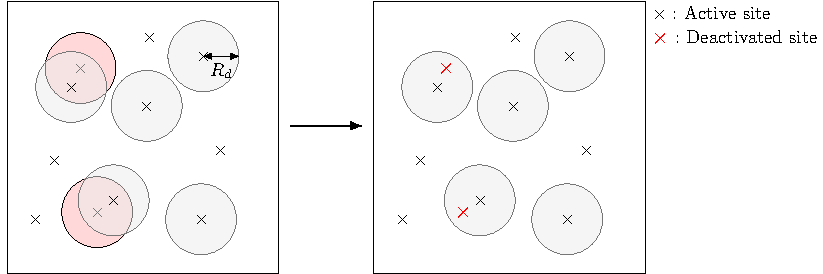
\includegraphics[width=0.9\linewidth]{img/site_interaction/static_suppression.pdf}
\caption{Sketch of the geometrical overlapping leading to static deactivation. Bubbles in red can not be accommodated on the surface due to their site laying below an existing bubble.}
\label{fig:static_deactivation}
\end{figure}


Thus, we need a correction of $N_{sit}$ to obtain the actual number of active sites $N_{sit,a}$ that can geometrically fit on the surface regarding the nucleation parameters. Given a bubble growth time before departure $t_{g,d}$ and an average nucleation frequency $f$, we can estimate the actual number of bubbles growing attached to their sites on the boiling surface as:

\begin{equation}
N_{b} = t_{g,d}\times f \times N_{sit,a} 
\end{equation}


If $N_{b}$ is used as an event density in the Poisson process, we can estimate the probability to have an undesired overlapping \ie two simultaneous bubbles of radius $R_{d}$ on neighboring sites at a distance $r\leq R_{d}$:

\begin{align}
\mathcal{P}\parth{r\leq R_{d}} &=1-\mathcal{P}\parth{N\parth{\pi R_{d}^{2}}=0} = 1-e^{-N_{sit,a}t_{g}f\pi R_{d}^{2}} = \mathcal{P}
\end{align}

This overlapping probability $\mathcal{P}$ can then be used to ponderate the number of sites given by the NSD correlation, yielding:

\begin{align}
&N_{sit,a}=\parth{1-\mathcal{P}}N_{sit} \\
%
\Leftrightarrow\  &N_{sit,a}t_{g,d}f\pi R_{d}^{2}e^{N_{b}t_{g,d}f \pi R_{d}^{2}}= N_{sit}t_{g,d}f \pi R_{d}^{2} \\
%
\Leftrightarrow\   &N_{sit,a} = \frac{\mathcal{W}\parth{N_{sit}{A_{sit}}}}{{A_{sit}}}
\label{eq:static_deact}
\end{align}
where $A_{sit}=t_{g,d}f \pi R_{d}^{2}$ and $\mathcal{W}$ is Lambert's W-function (reciprocal of $x \rightarrow xe^{x}$).

\begin{note*}{}
This calculation has originally been conducted by Gilman \cite{gilman_phd} and continued by Kommajosyula \cite{kommajosyula_development_2020}. 
\end{note*}

The evaluation of $\mathcal{W}$ can easily be achieved with a few iterations of a bisection method. Otherwise, Kommajosyula proposed an approximation to allow its direct computation \cite{kommajosyula_development_2020}.



\npar

On Figure \ref{fig:NSD_supp} we show the impact of the correction of Eq. \ref{eq:static_deact} on NSD correlations of Hibiki \& Ishii (Eq. \ref{eq:nsit_hibiki}) and Li \etal (Eq. \ref{eq:nsit_li}).



\subsection{Static coalescence}

Now that the actual number of bubble-generating sites have been identified, we can consider other interaction phenomena that can occur on the boiling surface. For instance, if two sites are simultaneously generating a bubble at a distance $d$ between $R_{d}$ and $2R_{d}$, the bubbles will coalesce while growing up to the detachment diameter. To estimate the probability of having a bubble on a site in this distance range, we consider the probability density function of the nearest-neighbour in the case of a homogeneous spatial Poisson process $f$ with an event density $\lambda$. 

\begin{align}
f\parth{r}=2\lambda \pi r e^{-\lambda \pi r^{2}}
\end{align} 

The considered probability of interaction is then :

\begin{align}
\mathcal{P}\parth{R_{d}\leq r \leq 2R_{d}} &=\int_{R_{d}}^{2R_{d}}f\parth{r} \mathrm{d}r \\
%
&= e^{-\lambda \pi R_{d}^{2}} - e^{-4\lambda \pi R_{d}^{2}}\\
%
&= e^{-\lambda \pi R_{d}^{2}}\crocht{1-\parth{e^{-\lambda \pi R_{d}^{2}}}^{3}} \\
&= \mathcal{P}_{coal,st} \ \ \ \text{with}\ \ \ \lambda=t_{g} f N_{b}
\end{align}

The density of bubble-generating sites that will lead to a static coalescence can then be estimated as :

\begin{align}
N_{coal,st}=\mathcal{P}_{coal,st}N_{b}
\end{align}

If we suppose that coalescing bubbles will instantly lift-off due to the perturbation associated with the coalescence process, this yields an associated boiling flux :

\begin{align}
\phi_{e,coal,st}=N_{coal,st} f \rho_{V}h_{LV} \frac{4}{3}\pi R_{coal,st}^{3} \ \ \ \text{where}\ \ \ R_{coal,st}=\sqrt[3]{2}R_{d} 
\end{align}

considering that the bubbles will merge approximately at $R=R_{d}$.

\subsection{Sliding coalescence}

Now that suppressed sites and sites that will lead to static coalescence have been identified, the remaining sites $N_{sl}=\parth{1-\mathcal{P}_{coal,st}}N_{b}$ will generate sliding bubbles. While sliding, a single bubble swipes an area :

\begin{align}
A_{sl, 1b} \approx l_{sl,1b}\frac{D_{d}+D_{lo}}{2}
\end{align}

In this area, there are an average number of bubble-generating sites $N_{b}A_{sl,1b}$ and an average number of growing bubbles on their sites $t_{g}f N_{b}A_{sl,1b}$

\npar
Two situations can happen from the sliding process :

\begin{itemize}
\item The bubble slides without coalescing
\item The bubble coalesces while sliding with a bubble growing on its site and lifts-off
\end{itemize}


Following the same approach from the static suppression, we can estimate the probability of finding no growing bubble over the sliding surface : 

\begin{align}
\mathcal{P}\parth{N\parth{A_{sl,1b}}=0 }=e^{-N_{b}t_{g}fA_{sl,1b}}
\end{align}

Thus, if a sliding bubble among the $N_{sl}$ does not encounter any growing bubble, the sites on its sliding area will be wiped and thus be quenched by cold liquid. This means that those sites will be suppressed due to the sliding of other bubbles over them.

Among the $N_{b}$ bubble generating sites we can identify 4 categories of sites :

\begin{itemize}
\item Sites generating bubbles which will slide without encountering any growing bubble on their path : $$N_{sl, NC}=N_{sl}e^{-ft_{g}N_{b}A_{sl,1b}}$$

\item Sites generating bubbles that will coalesce with a growing bubble during sliding : 
$$N_{sl, C}=  N_{sl}\parth{1-e^{-ft_{g}N_{b}A_{sl,1b}}}$$

\item Sites which will be suppressed by bubbles sliding without coalescing : $$N_{sup, sl}=N_{sl,NC}\ N_{b}A_{sl,1b}$$

\item Sites generating bubbles that will coalesce with a sliding bubble coming from upstream. Those bubbles are still in the growing phase up to detachment when they are coalescing with sliding bubbles. Therefore, there are equal to the number of sliding bubbles that will coalesce : $$N_{g,C}=N_{sl,C}$$

\end{itemize}

This allows to finally write :

\begin{align}
N_{b}&=N_{sl,NC}+N_{sl,C}+N_{sup,sl} + N_{g,C}\\
%
&=N_{sl}\crocht{2-e^{-ft_{g}N_{b}A_{sl,1b}}\parth{A_{sl,1b}N_{b}-1}}
\end{align}

Which finally yields the total number of sliding bubbles : 

\begin{align}
N_{sl}=\frac{N_{b}}{2-e^{-ft_{g}N_{b}A_{sl,1b}}\parth{A_{sl,1b}N_{b}-1}}
\end{align}
